\section{Object diffusion mini-protocol}

\definecolor{mygreen}{rgb}{0.109804,0.698039,0.341176}
\definecolor{myblue}{rgb}{0.360784,0.423529,255}

\usetikzlibrary{automata, positioning, arrows}
\usetikzlibrary{arrows,calc,matrix,shapes}

\tikzset{
    state/.style={
           rectangle,
           rounded corners,
           draw=black, very thick,
           minimum height=2em,
           inner sep=2pt,
           text centered,
           },
}

\newcommand{\header}[1]{\textbf{#1}}

\newcommand{\state}[1]{\texttt{#1}}
\newcommand{\trans}[1]{\texttt{#1}}
\newcommand{\msg}[1]{\textbf{\texttt{#1}}}

\newcommand{\Client}{\textcolor{mygreen}{\textbf{Client}}}
\newcommand{\Server}{\textcolor{myblue}{\textbf{Server}}}

\newcommand{\StInit}             {\state{StInit}}
\newcommand{\StIdle}{\state{StIdle}}
\newcommand{\StBusy}{\state{StBusy}}
\newcommand{\StDone}{\state{StDone}}
\newcommand{\StTxIdsBlocking}    {\state{StTxIdsBlocking}}
\newcommand{\StTxIdsNonBlocking} {\state{StTxIdsNonBlocking}}
\newcommand{\StTxs}              {\state{StTxs}}

\newcommand{\MsgInit}            {\msg{MsgInit}}
\newcommand{\MsgRequestTxIdsNB}  {\msg{MsgRequestTxIdsNonBlocking}}
\newcommand{\MsgRequestTxIdsB}   {\msg{MsgRequestTxIdsBlocking}}
\newcommand{\MsgReplyTxIds}      {\msg{MsgReplyTxIds}}
\newcommand{\MsgRequestTxs}      {\msg{MsgRequestTxs}}
\newcommand{\MsgReplyTxs}        {\msg{MsgReplyTxs}}
\newcommand{\MsgDone}{\msg{MsgDone}}

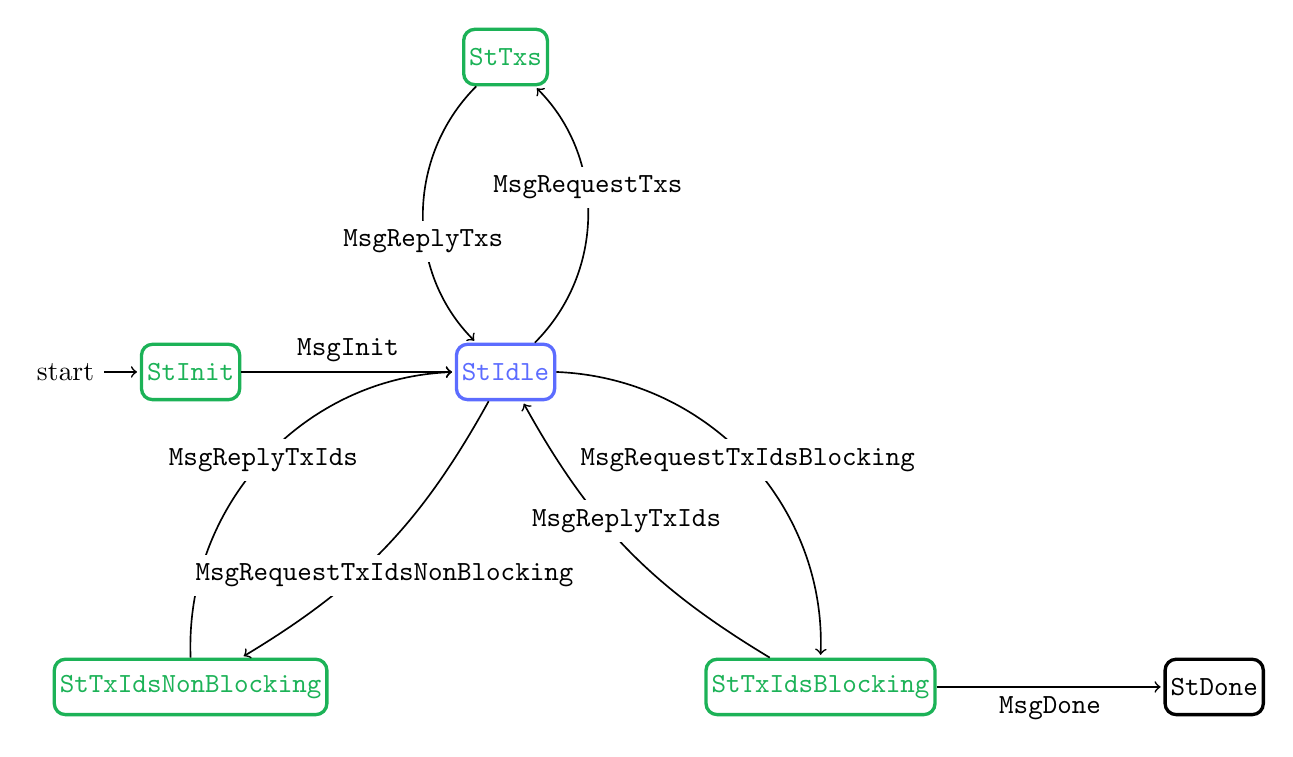
\begin{tikzpicture}[->,shorten >=1pt,auto,node distance=4.5cm, semithick]
  \tikzstyle{every state}=[fill=red,draw=none,text=white]
  \node[state, mygreen, initial] (I) at (-4,  0) {\StInit};
  \node[state, myblue]           (A) at ( 0,  0) {\StIdle};
  \node[state]                   (B) at ( 9, -4) {\StDone};
  \node[state, mygreen]          (C) at ( 4, -4) {\StTxIdsBlocking};
  \node[state, mygreen]          (D) at (-4, -4) {\StTxIdsNonBlocking};
  \node[state, mygreen]          (E) at ( 0,  4) {\StTxs};
  \draw (I)  edge[above]                    node[above]{\MsgInit}                                                (A);
  \draw (C)  edge[above]                    node[below]{\MsgDone}                                                (B);
  \draw (A)  edge[left, bend left=45]       node[fill = white, anchor = center]{\MsgRequestTxIdsB}               (C);
  \draw (C)  edge[right, bend left=15]      node[fill = white, anchor = center, above = 2pt]{\MsgReplyTxIds}     (A);
  \draw (D)  edge[right, bend left=45]      node[fill = white, anchor = center]{\MsgReplyTxIds}                  (A);
  \draw (A)  edge[right, bend left=15]      node[fill = white, anchor = center, below = 2pt]{\MsgRequestTxIdsNB} (D);
  \draw (A)  edge[left, bend right=45]      node[fill = white, anchor = center, above = 2pt]{\MsgRequestTxs}     (E);
  \draw (E)  edge[right,bend right=45]      node[fill = white, anchor = center, below = 2pt]{\MsgReplyTxs}       (A);
\end{tikzpicture}

\begin{figure}[h]
  \begin{center}
    \begin{tabular}{l|l}
      \header{state}      & \header{agency} \\\hline
      \StInit             & \Client \\
      \StIdle             & \Server \\
      \StTxIdsBlocking    & \Client \\
      \StTxIdsNonBlocking & \Client \\
      \StTxs              & \Client \\
    \end{tabular}
    \caption{Tx-Submission state agencies}
  \end{center}
\end{figure}

\paragraph{Protocol messages}
\begin{description}
\item [\MsgInit] initial message of the protocol
\item [\MsgRequestTxIdsNB{} {\boldmath $(ack,req)$}]
      The server asks for new transaction ids and acknowledges old ids.
      The client immediately replies (possibly with an empty list).
\item [\MsgRequestTxIdsB{} {\boldmath $(ack,req)$}]
      The server asks for new transaction ids and acknowledges old ids.
      The client will block until new transactions are available.
\item [\MsgReplyTxIds{} {\boldmath ($\langle (id, size) \rangle$) }]
      The client replies with a list of available transactions.
      The list contains pairs of transaction ids and the corresponding size of the transaction in bytes.
      In the blocking case, the reply is guaranteed to contain at least one transaction.
      In the non-blocking case, the reply may contain an empty list.
\item [\MsgRequestTxs{} {\boldmath ($\langle ids \rangle$)}]
      The server requests transactions by sending a list of transaction-ids.
\item [\MsgReplyTxs{} {\boldmath ($\langle txs \rangle$})]
      The client replies with a list of transactions.
\item [\MsgDone]
      The client terminates the mini protocol.
\end{description}

\begin{table}[h]
  \begin{tabular}{l|l|l|l}
    \header{from state} & \header{message}    & \header{parameters}           & \header{to state}   \\\hline
    \StInit             & \MsgInit            &                               & \StIdle             \\
    \StIdle             & \MsgRequestTxIdsNB  & $ack$,$req$                   & \StTxIdsNonBlocking \\
    \StIdle             & \MsgRequestTxIdsB   & $ack$,$req$                   & \StTxIdsBlocking    \\
    \StTxIdsNonBlocking & \MsgReplyTxIds      & $\langle (id, size) \rangle$  & \StIdle             \\
    \StTxIdsBlocking    & \MsgReplyTxIds      & $\langle (id, size) \rangle$  & \StIdle             \\
    \StIdle             & \MsgRequestTxs      & $\langle ids \rangle$         & \StTxs              \\
    \StTxs              & \MsgReplyTxs        & $\langle txs \rangle$         & \StIdle             \\
    \StIdle             & \MsgDone            &                               & \StDone             \\
  \end{tabular}
  \caption{Tx-Submission mini-protocol (version 2) messages.}
\end{table}

\subsection{Size limits per state}

Table~\ref{table:tx-submission-size-limits} specifies how many bytes can be sent
in a given state; indirectly, this limits the payload size of each message.  If
a space limit is violated, the connection SHOULD be torn down.

\begin{table}[h]
  \begin{center}
    \begin{tabular}{l|r}
      \header{state}      & \header{size limit in bytes} \\\hline
      \StInit             & \texttt{5760} \\
      \StIdle             & \texttt{5760} \\
      \StTxIdsBlocking    & \texttt{2500000} \\
      \StTxIdsNonBlocking & \texttt{2500000} \\
      \StTxs              & \texttt{2500000} \\
    \end{tabular}
    \caption{size limits per state}
    \label{table:tx-submission-size-limits}
  \end{center}
\end{table}

\subsection{Timeouts per state}

The table~\ref{table:tx-submission-timeouts} specifies message timeouts in
a given state.  If a timeout is violated, the connection SHOULD be torn down.

\begin{table}[h]
  \begin{center}
    \begin{tabular}{l|r}
      \header{state}      & \header{timeout} \\\hline
      \StInit             & - \\
      \StIdle             & - \\
      \StTxIdsBlocking    & - \\
      \StTxIdsNonBlocking & \texttt{10}s \\
      \StTxs              & \texttt{10}s \\
    \end{tabular}
    \caption{timeouts per state}
    \label{table:tx-submission-timeouts}
  \end{center}
\end{table}

\subsection{CDDL encoding specification}\label{tx-submission2-cddl}

\lstset{
  xleftmargin=2pt,
  stepnumber=1,
  belowcaptionskip=\bigskipamount,
  captionpos=b,
  escapeinside={*'}{'*},
  language=haskell,
  tabsize=2,
  emphstyle={\bf},
  commentstyle=\it,
  stringstyle=\mdseries\rmfamily,
  showspaces=false,
  keywordstyle=\bfseries\rmfamily,
  columns=flexible,
  basicstyle=\small\sffamily,
  showstringspaces=false,
  morecomment=[l]\%,
}
\lstdefinelanguage{cddl}{
  morekeywords={bool,uint,nint,int,float16,float32,float64,float,bstr,bytes,tstr,text},
  morecomment=[l]{;},
  morestring=[b]",
}
\lstdefinestyle{cddl}{
  numbers=left,
  language=cddl,
  columns=fixed,
}

%% NOTE: lst imports are relative to the main file, hence the necessary
%% `protocol-changes/` prefix.
\lstinputlisting[style=cddl]{protocol-changes/object-diffusion.cddl}

\subsection{Client and Server Implementation}

The protocol has two design goals: It must diffuse transactions with high efficiency
and, at the same time, it must rule out
asymmetric resource attacks from the transaction consumer against the transaction provider.

The protocol is based on two pull-based operations.
The transaction consumer can ask for a number of transaction ids, and it can use these
transaction ids to request a batch of transactions.
The transaction consumer has flexibility in the number of transaction ids it requests,
whether to actually download the transaction body
and flexibility in how it batches the download of transactions.
The transaction consumer can also switch between requesting transaction ids and downloading
transaction bodies at any time.
It must, however, observe several constraints that are necessary for a memory-efficient implementation
of the transaction provider.

Conceptually, the provider maintains a limited size FIFO of outstanding transactions per consumer.
(The actual implementation can, of course, use the data structure that works best).
The maximum FIFO size is a protocol parameter.
The protocol guarantees that, at any time, the consumer and producer agree on the current size of
that FIFO and on the outstanding transaction ids.
The consumer can use a variety of heuristics to request transaction ids and transactions.
One possible implementation for a consumer is to maintain a FIFO that mirrors the producer's FIFO
but only contains the transaction ids (and the size of the transaction) and not the full transactions.

After the consumer requests new transaction ids, the provider replies with a list of transaction ids and
puts these transactions in its FIFO.
As part of a request, a consumer also acknowledges the number of old transactions,
which are removed from the FIFO at the same time.
The provider checks that the size of the FIFO, i.e. the number of outstanding transactions,
never exceeds the protocol limit and aborts the connection if a request violates the limits.
The consumer can request any batch of transactions from the current FIFO in any order.
Note, however, that the reply will omit any transactions that have become invalid in the meantime.
(More precisely, the server will omit invalid transactions from the reply, but they will still be counted in the FIFO
size, and they will still require an acknowledgement from the consumer).

The protocol supports blocking and non-blocking requests for new transactions ids.
If the FIFO is empty, the consumer must use a blocking request; otherwise, it must be a non-blocking request.
The producer must reply immediately (i.e. within a small timeout) to a non-blocking request.
It replies with not more than the requested number of ids (possibly with an empty list).
A blocking request, on the other side, waits until at least one transaction is available.
